
\item Two conducting cylinders of equal length but different radii are connected in series between two heat baths kept at temperatures \(T_1 = 300 \, K\) and \(T_2 = 100 \, K\), as shown in the figure. The radius of the bigger cylinder is twice that of the smaller one and the thermal conductivities of the materials of the smaller and the larger cylinders are \(K_1\) and \(K_2\) respectively. If the temperature at the junction of the two cylinders in the steady state is \(200 \, K\), then \(K_1/K_2 = \) \underline{\hspace{2cm}}.
\begin{center}
    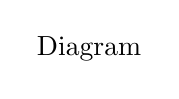
\begin{tikzpicture}
        \node {Diagram};
    \end{tikzpicture}
\end{center}
